25. \begin{figure}[ht!]
\center{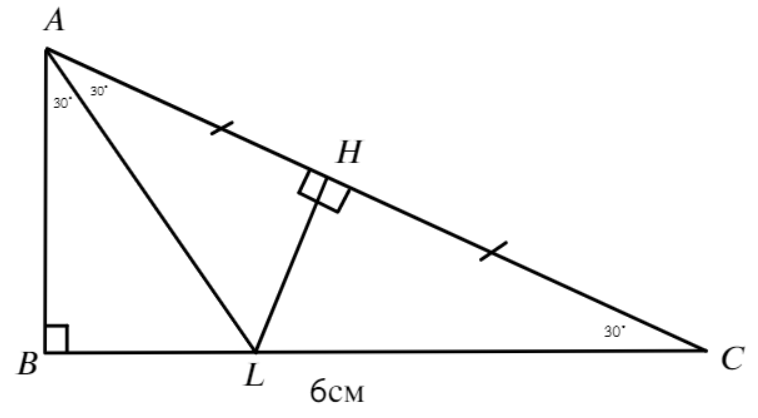
\includegraphics[scale=0.35]{g25.png}}
\end{figure}\\
Так как $AL$ является биссектрисой, $\angle BAL=\angle LAC=60^\circ:2=30^\circ.$ Угол $C$ также равен $90^\circ-\angle A=90^\circ-60^\circ=30^\circ.$ В прямоугольных треугольниках $LAH$ и $LCH$ катет $LH$ лежит напротив угла в $30^\circ,$ а значит $AL=LC=2LH.$ В прямоугольном треугольнике $ABL$ катет $BL$ лежит напротив угла
в $30^\circ,$ а значит $BL=AL:2=2LH:2=LH.$ Таким образом, $BC=BL+LC=LH+2LH=3LH=6$см, откуда $LH=6:3=2$см.\newpage\noindent
